\documentclass[compress]{beamer}

\usepackage{german}
\usepackage{url}

\title{Phasing out UNIX before 2038-01-19}
\subtitle{UNIX and C are obsolete}

\author{Andreas Bogk and Hannes Mehnert}

\begin{document}
\date{What The Hack, 29.7.2005}
\frame{\titlepage}

\begin{frame}
  \frametitle{Overview}
  \begin{itemize}
  \item problems with C
  \item requirements for a replacement
  \item master plan for phasing out UNIX
  \item dylan programming language
  \end{itemize}
\end{frame}

\begin{frame}
  \frametitle{Why C sucks}
  \begin{itemize}
  \item buffer overflows
  \item integer overflows
  \item format string vulnerabilities
  \item access to already freed memory
  \end{itemize}
  These bug classes make up the vast majority of the security problems registered at CVE!
\end{frame}

\begin{frame}[fragile]
  \frametitle{Buffer overflows}
  \begin{verbatim}
void foo(char* somestring) {
    char buffer[32];

    strcpy(buffer, somestring);
}
  \end{verbatim}
  And what happens if ``somestring'' is longer than 31 characters?
\end{frame}

\begin{frame}[fragile]
  \frametitle{Integer overflows}
  \begin{verbatim}
    char buffer[MAXLEN];
    int counter = 0;

    while(!eof(input)) {
        char c = getc(input);
        counter++;
    }

    if (counter < MAXLEN) {
        rewind(input);
        read(buffer, input, counter);
    }
  \end{verbatim}
  This only works if ``counter'' is less than $2 ^ {32} - 1$...
\end{frame}

\begin{frame}[fragile]
  \frametitle{Format string vulnerability}
  \begin{verbatim}
    void foo(char* somestring) {
        printf(somestring);
    }
  \end{verbatim}
  What happens if ``somestring'' contains a \%? varargs are not type safe!
\end{frame}

\begin{frame}[fragile]
  \frametitle{Double Free}
  \begin{verbatim}
    char* buffer = malloc(strlen(somestring));
    ...
    free(buffer);
    ...
    strcpy(buffer, somestring);
    ...
    malloc();
  \end{verbatim}
  malloc has free memory in a double linked list, it stores the pointers only in the free block.
\end{frame}

\begin{frame}
  \frametitle{Real programmers don't make mistakes!}
  \begin{itemize}
  \item experience reveals: everyone make mistakes
  \item the real problem: in C bugs are vulnerabilities
  \item and C++ and Objective C are not better!
  \end{itemize}
\end{frame}

\begin{frame}
  \frametitle{Possible workarounds}
  \begin{itemize}
  \item better QA procedures
  \item source code reviews
  \item automated analysis of binaries
  \item virtualisation
  \end{itemize}
  Those workarounds are expensive, hard to do,
  slow down development process.
\end{frame}

\begin{frame}
  \frametitle{Solutions}
  technical solutions:
  \begin{itemize}
  \item bounds checking
  \item integer overflow checking
  \item strong typing
  \item garbage collection
  \end{itemize}
  Bugs are caught without endangering semantical integrity
  of the language and therefore the security of the system.
  Minimizing the trusted computing base happens on semantical layer.

  The only place C belongs to is the museum!
\end{frame}

\begin{frame}
  \frametitle{But all languages are Turing equivalent!}
  \begin{itemize}
  \item programming languages are used for communication between human beings
  \item instructions for machines are side effects
  \item different languages have different expressive powers
  \end{itemize}
  ... who still programs in assembler with a hex editor? programming languages are not all the same. The choice is not arbitrary.
\end{frame}

\begin{frame}
  \frametitle{Security is more than bounds checks}
  readable, abstract code is understandable, maintainable, testable code
  This is the prerequisite for secure code!
\end{frame}

\begin{frame}
  \frametitle{Why UNIX sucks}
  \begin{itemize}
  \item kernel vs userland
  \item monolithic kernel
  \item process model
  \item hard to debug
  \end{itemize}
\end{frame}

\begin{frame}
  \frametitle{Lisp machines - history}
  \begin{itemize}
  \item developed at MIT
  \item handbook was written by Richard Stallman
  \item later commercialy sold
  \item even though the system came with complete source code, it was not free software
  \end{itemize}
\end{frame}

\begin{frame}
  \frametitle{Lisp machines}
  \begin{itemize}
  \item whole OS written in lisp
  \item single address space
  \item CPU has tag bits, each pointer is tagged with its type
  \item auto-forwarding pointers for faster garbage collection
  \end{itemize}
\end{frame}

\begin{frame}
  \frametitle{Our Vision}
  Phasing out UNIX before 2038-01-19! Rewrite everything from scratch!
\end{frame}

\begin{frame}
  \frametitle{A little more realistic}
  \begin{itemize}
  \item lots of legacy applications, which we can't get rid of
  \item coexistence of UNIX and a secure environment
  \item e.g. L4 Micro-Kernel, L4Linux as a process
  \item but: secure environment written in a secure language
  \item especially hardware drivers, IP, crypto
  \end{itemize}
  The penguin may play in a sandbox, where it can't break anything.
\end{frame}

\begin{frame}
  \frametitle{Possible scenarios}
  \begin{itemize}
  \item management for cryptographic keys
  \item network services
  \item secure console
  \end{itemize}
  Desktop environment can't be rewritten so fast (lots of code).
\end{frame}

\begin{frame}
  \frametitle{Requirements for programming languages}
  \begin{itemize}
  \item universal
  \item powerful
  \item easy to learn
  \item performant
  \item easy to read
  \item open source implementation
  \item tools (debugger, profiler, IDE)
  \item libraries, frameworks
  \item secure!
  \end{itemize}
\end{frame}

\begin{frame}
  \frametitle{History of Dylan}
  \begin{itemize}
  \item dialect of lisp
  \item Ralph, the programming language for Apple Newton
  \item Apple, CMU, Harlequin
  \item Dylan Interim Reference Manual
  \item Dylan Reference Manual (DRM)
  \end{itemize}
  since DRM no longer prefix (lisp) syntax
\end{frame}

\begin{frame}
  \frametitle{Apple Dylan}
  \begin{itemize}
  \item technology release (based on MCL)
  \item Apple Cambridge labs
  \item implementation on 68k, later PowerPC
  \item 1996 abandoned for lack of money
  \end{itemize}
\end{frame}

\begin{frame}
  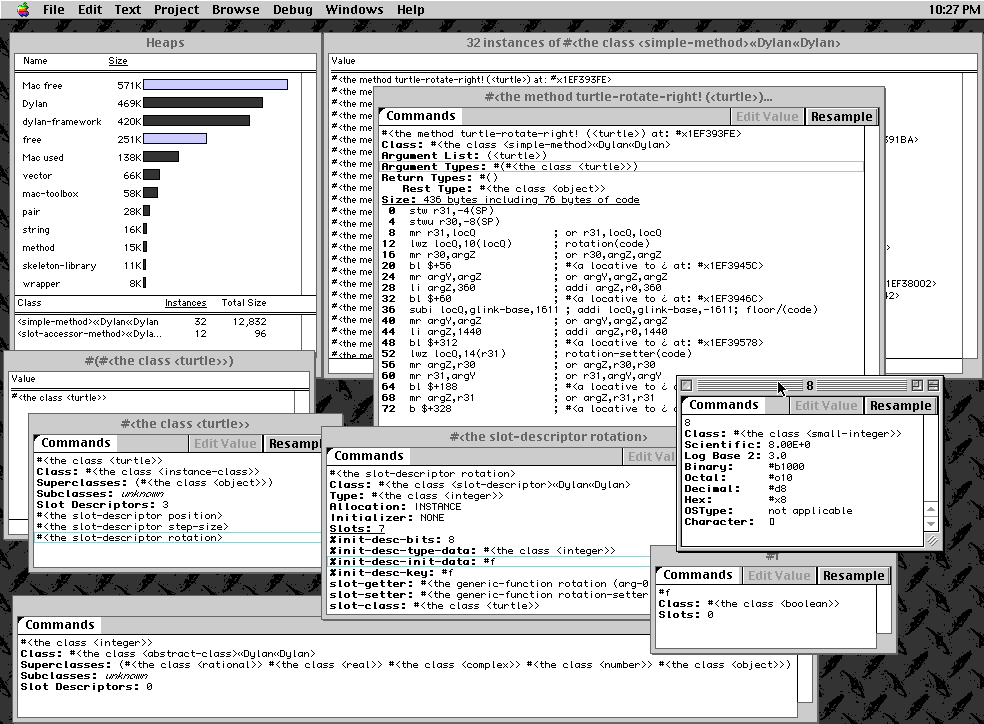
\includegraphics [height=\textheight, width=\textwidth]{appledylan-debugging-grab-bag.png}
\end{frame}

\begin{frame}
  \frametitle{CMU}
  \begin{itemize}
  \item gwydion project
  \item goal: development environment
  \item DARPA funded between 1994 and 1998
  \item dylan interpreter in C
  \item dylan compiler to C written in dylan
  \item since 1994 open source license (mostly BSD)
  \item since 1998 open development process
  \end{itemize}
\end{frame}

\begin{frame}
  \frametitle{Harlequin}
  \begin{itemize}
  \item dylan compiler written in dylan
  \item developers had many experience (lisp machine, LispWorks)
  \item native compiler with IDE (only on win32 so far)
  \item debugger, profiler, interactor, hot code update
  \item command line compiler for linux/x86
  \item originally a commercial development, since 2004 open source license (LGPL)
  \item large scale professional development (30 person years work just for the garbage collector)
  \end{itemize}
\end{frame}

\begin{frame}
  \frametitle{Existing libraries}
  \begin{itemize}
  \item DUIM (Dylan User Interface Manager)
  \item corba (2.0, some 2.2 features)
  \item ODBC
  \item network
  \item regular expressions
  \item dood (persistent object store)
  \item file system
  \item XML parser
  \item C interfaces to png, pdf, postgresql, sdl, opengl
  \item stand alone web server and proof of concept wiki
  \item ...
  \end{itemize}
\end{frame}

%\begin{frame}
%  \begin{itemize}
%  \item Einordnung in Programmiersprachen
%  \end{itemize}
%\end{frame}

\begin{frame}[fragile]
  \frametitle{Syntax}
Algol like syntax:
  \begin{verbatim}
begin
  for (i from 0 below 9)
    format-out("Hello world");
  end for;
end
  \end{verbatim}
\end{frame}

\begin{frame}
  \frametitle{Naming Conventions}
  \begin{itemize}
  \item allowed in names: +=-*$<>$
  \item - instead of \_
  \item classes begin and end with angle brackets: $<$number$>$
  \item global variables begin and end with asterisks: *machine-state*
  \item program constants begin with a dollar sign: \$pi
  \item predicate functions end with a question mark: even?
  \item destructive functions end with exclamation mark: reverse!
  \item getters and setters: element element-setter
  \end{itemize}
\end{frame} 

\begin{frame}
  \frametitle{Dynamically and strongly typed}
  \begin{itemize}
  \item strong vs weak typing
  \item static vs dynamic typing
  \end{itemize}
\end{frame}

\begin{frame}
  \frametitle{Object oriented}
  \begin{itemize}
  \item class based object system
  \item everything is inherited from class $<$object$>$
  \item multiple inheritance, but the right way: superclass linearization
  \item difference to widely deployed object oriented programming languages: functions are not part of classes
  \end{itemize}
\end{frame}

\begin{frame}[fragile]
  \frametitle{Class definition}
  \begin{verbatim}
define class <square> (<rectangle>)
  slot x :: <number> = 0, init-keyword: x:;
  slot y :: <number> = 0, init-keyword: y:;
  constant slot width :: <number>,
     required-init-keyword: width:;
end class;  
  \end{verbatim}
\end{frame}

%\begin{frame}
%  \begin{itemize}
%  \item Garbage collection
%  \end{itemize}
%\end{frame}

\begin{frame}[fragile]
  \frametitle{Keyword arguments}
  \begin{verbatim}
define function describe-list
    (my-list :: <list>, #key verbose?) => ()
  format(*standard-output*,
         "{a <list>, size: %d",
         my-list.size);
  if (verbose?)
    format(*standard-output*, ", elements:");
    for (item in my-list)
      format(*standard-output*, " %=", item);
    end for;
  end if;
  format(*standard-output*, "}");
end function;
  \end{verbatim}
\end{frame}

\begin{frame}
  \frametitle{Higher order functions}
  \begin{itemize}
  \item anonymous functions (lambda calculus)
  \item closures
  \item curry, reduce, map, do
  \item function composition
  \end{itemize}
\end{frame}

\begin{frame}[fragile]
  \frametitle{Anonymous functions and closures}
  \begin{verbatim}
define function make-linear-mapper
    (times :: <integer>, plus :: <integer>)
 => (mapper :: <function>)
  method (x)
    times * x + plus;
  end method;
end function;

define constant times-two-plus-one =
  make-linear-mapper(2, 1);

times-two-plus-one(5);
// Returns 11.
  \end{verbatim}
\end{frame}

\begin{frame}[fragile]
  \frametitle{Curry, reduce, map}
  \begin{verbatim}
let printout = curry(print-object, *standard-output*);
do(printout, #(1, 2, 3));

reduce(\+, 0, #(1, 2, 3)) // returns 6

reduce1(\+, #(1, 2, 3)) //returns 6

map(\+, #(1, 2, 3), #(4, 5, 6))
 //returns #(5, 7, 9)
  \end{verbatim}
\end{frame}

\begin{frame}[fragile]
  \frametitle{Function composition, interfacing to C}
  \begin{verbatim}
define interface
  #include "ctype.h",
    import: {"isalpha" => is-alphabetic?,
	     "isdigit" => is-numeric?},
    map: {"int" => <boolean>};
end interface;

define constant is-alphanumeric? =
  disjoin(is-alphabetic?, is-numeric?);
  \end{verbatim}
\end{frame}

\begin{frame}[fragile]
  \frametitle{Generic functions}
  \begin{verbatim}
define method double
    (s :: <string>) => result
  concatenate(s, s);
end method;

define method double
    (x :: <number>) => result
  2 * x;
end method;
  \end{verbatim}
\end{frame}

\begin{frame}[fragile]
  \frametitle{Multiple dispatch}
  \begin{footnotesize}
  \begin{verbatim}
define method inspect-vehicle
  (vehicle :: <vehicle>, i :: <inspector>) => ();
  look-for-rust(vehicle);
end;
define method inspect-vehicle
    (car :: <car>, i :: <inspector>) => ();
  next-method(); // perform vehicle inspection
  check-seat-belts(car);
end;
define method inspect-vehicle
    (truck :: <truck>, i :: <inspector>) => ();
  next-method(); // perform vehicle inspection
  check-cargo-attachments(truck);
end;
define method inspect-vehicle
    (car :: <car>, i :: <state-inspector>) => ();
  next-method(); // perform car inspection
  check-insurance(car);
end;
  \end{verbatim}
  \end{footnotesize}
\end{frame}

\begin{frame}[fragile]
  \frametitle{Optional type restrictions of bindings}
  \begin{verbatim}
define method foo
    (a :: <number>, b :: <number>)
  let c = a + b;
  let d :: <integer> = a * b;
  c := "foo";
  d := "bar"; // Type error!
end
  \end{verbatim}
  Serves on the one hand as assert, on the other hand type inference.
\end{frame}

\begin{frame}[fragile]
  \frametitle{Macros}
  \begin{verbatim}
define macro with-open-file
  { with-open-file (?stream:variable = ?locator:expression,
                    #rest ?keys:expression)
      ?body:body
    end }
  => { begin
         let ?stream = #f;
         block ()
           ?stream := open-file-stream(?locator, ?keys);
           ?body
         cleanup
           if (?stream & stream-open?(?stream))
             close(?stream)
           end;
         end
       end }
end macro with-open-file;
  \end{verbatim}
\end{frame}


%warum das performt

\begin{frame}[fragile]
  \frametitle{A simple for-loop...}
  \begin{verbatim}
let collection = #[1, 2, 3];
for (i in collection)
  format-out("%=\n", i);
end for;
  \end{verbatim}
\end{frame}

\begin{frame}[fragile]
  \frametitle{... is in real a macro with iterator ...}
  \begin{verbatim}
let (initial-state, limit, next-state, finished-state?,
     current-key, current-element) =
  forward-iteration-protocol(collection);
local method repeat (state)
   block (return)
     unless (finished-state?(collection, state, limit))
       let i = current-element(collection, state);
       format-out("%=\n", i);
       repeat(next-state(collection, state));
     end unless;
   end block;
 end method;
repeat(initial-state)
  \end{verbatim}
\end{frame}

\begin{frame}[fragile]
  \frametitle{... which gets optimized to a simple loop.}
  \begin{footnotesize}
  \begin{verbatim}
while (1) {
  if ((L_state < 3)) {
    L_PCTelement = SLOT((heapptr_t)&literal_ROOT,
                        descriptor_t,
                        8 + L_state_2 * sizeof(descriptor_t));
    [...]
    L_state = L_state + 1;
  } else {
    goto block0;
  }
}
block0:;
  \end{verbatim}
  \end{footnotesize}
\end{frame}

\begin{frame}[fragile]
  \frametitle{Type unions}
  \begin{verbatim}
define constant <green-thing> =
  type-union(<frog>, <broccoli>);

define constant kermit = make(<frog>);

define method red?(x :: <green-thing>)
  #f
end;

red?(kermit) => #f
  \end{verbatim}
\end{frame}

\begin{frame}[fragile]
  \frametitle{False-or, singleton}
  \begin{verbatim}
type-union(singleton(#f, type)) == false-or(type)

define method find-foo (x) => (index :: false-or(<integer>))
 ... //returns index if found, false if not found
end method say;

type-union(symbol1, symbol2) == one-of(symbol1, symbol2)
define method say (x :: one-of(#"red", #"green", #"blue"))
  ...
end method say;
  \end{verbatim}
\end{frame}


\begin{frame}[fragile]
  \frametitle{Nonlocal exits}
  \begin{verbatim}
block (return)
  open-files();
  if (something-wrong)
    return("didn't work");
  end if;
  compute-with-files()
cleanup
  close-files();
end block
  \end{verbatim}
\end{frame}

\begin{frame}[fragile]
  \frametitle{Exceptions}
  \begin{verbatim}
block ()
  open-files();
  compute-with-files()
exception (<error>) 
  "didn't work";
cleanup
  close-files();
end block
  \end{verbatim}
\end{frame}

\begin{frame}[fragile]
  \frametitle{Library and Module}
  \begin{verbatim}
define library hello-world
  use dylan, import: all;
  use io, import: { format-out };
  export hello-world;
end library;

define module hello-world
  use dylan;
  use format-out;
  export say-hello;
end module;
  \end{verbatim}
\end{frame}

\begin{frame}
  \frametitle{Links}
  \begin{itemize}
  \item WWW: \url{http://www.gwydiondylan.org/}
  \item Dylan Programming: \url{http://www.gwydiondylan.org/books/dpg/}
  \item Dylan Reference Manual: \url{http://www.gwydiondylan.org/books/drm/}
  \item IRC: irc.freenode.net, \#dylan
  \item mailing list: gd-hackers@gwydiondylan.org
  \end{itemize}
\end{frame}

\end{document}
